\lab{Algorithms}{The Finite Element method}{The Finite Element method}
\label{lab:FEM}

The equation we will solve is 
\begin{align}
	\begin{split}
	&{ }\epsilon y'' - y' = f(x),\\
	&{ }y(0) = \alpha, \quad y(1) = \beta . 
	\end{split}\label{FEM:eqn1}
\end{align}
The solution $u$ of \eqref{FEM:eqn1} lies in some appropriate function space $V$.%; in any case, we can approximate it arbitrarily well in $C^0[0,1]$ by a piecewise linear function. 


Let $w$ be a test function; that is, suppose $w$ is infinitely differentiable and satisfies
$w(0) = w(1) = 0$. We multiply \eqref{FEM:eqn1} by $w$ and integrate over $[0,1]$ to obtain 
\begin{align*}
	&{ } \int_0^1 \epsilon y''w - y'w = \int_0^1 f w, \\
	&{ } \int_0^1 -\epsilon y'w' - y'w = \int_0^1 f w.
\end{align*}
Rather than trying to solve \eqref{FEM:eqn1}, we instead consider the problem of solving the equation 
\begin{align}
	a(y,w) &= l(w), \quad \forall \, w \in V,
	\label{FEM:integral_form}
\end{align}
where $a$ is a bilinear function on $V$ defined by $a(y,w) = \int_0^1 -\epsilon y'w' - y'w$, and $l$ is a the linear function given by $l(w) = \int_0^1 f w$.  \eqref{FEM:integral_form} is called the weak integral formulation of \eqref{FEM:eqn1}.




Let $\mathrm{P}_n$ be some partition $0 = x_0 < x_1< \ldots < x_{n} = 1$ of $[0,1]$, and let $V_n$ be the finite-dimensional vector space of continuous functions $v$ on $[0,1]$ where $v|_{[{x_j,x_{j+1}}]}$ is linear for $0 \leq j \leq n-1$. The intervals $[{x_j,x_{j+1}}]$ are the finite elements used in this method.  $V_n$ has dimension $n+1$, since there are $n+1$ degrees of freedom for continuous piecewise linear functions in $V$. Let $V_{0n}$ be the subspace of $V_n$ of dimension $n-1$ whose elements are zero at the endpoints of $[0,1]$. 
Let $\triangle x_n = \max_{0 \leq j \leq n-1}|x_{j+1} - x_j|$. 

Let $\{\mathrm{P}_n\}$ be a sequence of partitions that are refinements of each other, such that $\triangle x_n \to 0$ as $n \to \infty$. Then in particular we have that $V_1 \subset V_2 \subset \ldots \subset V_n \ldots \subset V$.  For each partition $\mathrm{P}_n$ we can look for an approximation $u_n(x) \in V_n$ for the true solution $u(x)$; if we do this correctly then $u_n(x) \to u(x)$ as $n$ gets large. 


Consider a partion $\mathrm{P}_5 = \{x_0, x_1, \ldots, x_5\}$. We will define some basis functions $\phi_i$, $i = 0, \ldots, 5$ for the corresponding vector space $V_5$. For $i = 1, \ldots, 4$, let $\phi_i$ be the hat function given by 
\[
\phi_i(x) = \begin{cases}
(x - x_{i-1})/h_i \quad \text{ if } x \in [x_{i-1},x_i]\\
 (x_{i+1} - x)/h_{i+1} \quad \text{ if } x \in [x_{i},x_{i+1}]\\
0 \quad \text{ otherwise}
\end{cases}
\]
where $h_i = x_i - x_{i-1}$; see Figures \ref{FEM:one_basis_function} and \ref{FEM:basis_functions}.

We look for an approximation $\hat{y} = \sum_{i=0}^5 k_i \phi_i \in V_5$ of the true solution $y$; that is, we need to find appropriate values for the constants $k_i$. We impose the condition on $\hat{y}$ that 
\[a(\hat{y},w) = l(w) \quad \forall \, w \in V_{05}.\]
Equivalently, we require that 
\[a \left( \sum_{i=0}^5 k_i \phi_i,\phi_j \right) = l(\phi_j) \quad \text{for } j = 1,2,3,4,\]
since $\phi_1, \phi_2, \phi_3, \phi_4$ form a basis for $V_{05}$.


Since $a$ is bilinear, we obtain 
\[
\sum_{i=0}^5 k_i  a ( \phi_i,\phi_j ) = l(\phi_j) \quad \text{for } j = 1,2,3,4
\]
To satisfying the boundary conditions, we also require that $k_0 = \alpha$, $k_5 = \beta$.
These equations can be written in matrix form as 
\begin{align} AK = \Phi,\label{FE:linear_system}\end{align}
where 
\[
A = \left[\begin{array}{cccccc}1 & 0 & 0 & 0 & 0 & 0 \\a(\phi_0,\phi_1) & a(\phi_1,\phi_1) & a(\phi_2,\phi_1) & 0 & 0 & 0 \\0 & a(\phi_1,\phi_2) & a(\phi_2,\phi_2) & a(\phi_3,\phi_2) & 0 & 0 \\0 & 0 & a(\phi_2,\phi_3) & a(\phi_3,\phi_3) & a(\phi_4,\phi_3) & 0 \\0 & 0 & 0 & a(\phi_3,\phi_4) & a(\phi_4,\phi_4) & a(\phi_5,\phi_4) \\0 & 0 & 0 & 0 & 0 &1\end{array}\right]
\]
and
\[
K = \left[\begin{array}{c}k_0 \\k_1 \\k_2 \\k_3 \\k_4 \\k_5\end{array}\right] , \quad\Phi =  \left[\begin{array}{c}\alpha \\l(\phi_1) \\l(\phi_2) \\l(\phi_3) \\l(\phi_4) \\\beta\end{array}\right] .
\]

Note that $a(\phi_i,\phi_j) = 0$ for most values of $i, j$ (that is, when the hat functions do not have overlapping domains).  Thus the finite element method usually results in a sparse linear system. 
To compute the coefficients of \eqref{FE:linear_system} we begin by evaluating some integrals. Since
\[
\phi_i'(x) = \begin{cases}
1/h_i \quad \quad \quad \, \text{for } x_{i-1} < x < x_i,\\
 -1/h_{i+1} \quad \text{ for } x_{i} < x < x_{i+1},\\
0 \quad \quad \quad \quad \, \text{ otherwise},
\end{cases}
\]
we obtain  
\begin{align*}
\int_0^1  \phi_i'\phi_j' &= \begin{cases}
- 1/h_{i+1} \quad \quad \quad \text{ if } j=i+1,\\
1/h_i + 1/h_{i+1} \quad \text{if } j=i,\\
0 \quad \quad \quad \quad \quad \quad \, \text{ otherwise},
\end{cases} \\
\int_0^1  \phi_i'\phi_j &= \begin{cases}
- 1/2 \quad \,\text{ if } j=i+1,\\
1/2 \quad \quad \text{ if } j=i-1,\\
0 \quad \text{ otherwise},
\end{cases} \\
l(\phi_j) &= (1/2)(h_j + h_{j+1}) , \\
a(\phi_i,\phi_j) &= \begin{cases}
\epsilon/h_{i+1} + 1/2 \quad \quad \, \text{ if } j=i+1,\\
-\epsilon/h_i -\epsilon/h_{i+1} \quad  \text{ if } j=i,\\
\epsilon/h_i - 1/2 \quad \quad \quad \, \text{ if } j=i-1,\\
0 \quad \text{ otherwise}
\end{cases}
\end{align*}
We may now solve \eqref{FE:linear_system} using any standard linear solver. 
% \begin{align*}
% 
% \end{align*}

% \begin{align}
% \left[\begin{array}{cccccc}1 & 0 & 0 & 0 & 0 & 0 \\-\epsilon/h_1 & \epsilon/h_1 + \epsilon/h_2 & -\epsilon/h_2 & 0 & 0 & 0 \\0 & -1/h_2 & a(\phi_2,\phi_2) & a(\phi_3,\phi_2) & 0 & 0 \\0 & 0 & a(\phi_2,\phi_3) & a(\phi_3,\phi_3) & a(\phi_4,\phi_3) & 0 \\0 & 0 & 0 & a(\phi_3,\phi_4) & a(\phi_4,\phi_4) & a(\phi_5,\phi_4) \\0 & 0 & 0 & 0 & 0 &1\end{array}\right]
% \left[\begin{array}{c}k_0 \\k_1 \\k_2 \\k_3 \\k_4 \\k_5\end{array}\right] = \left[\begin{array}{c}\alpha \\l(\phi_1) \\l(\phi_2) \\l(\phi_3) \\l(\phi_4) \\\beta\end{array}\right] \label{FE:linear_system}
% \end{align}






\begin{figure}[ht]
\centering
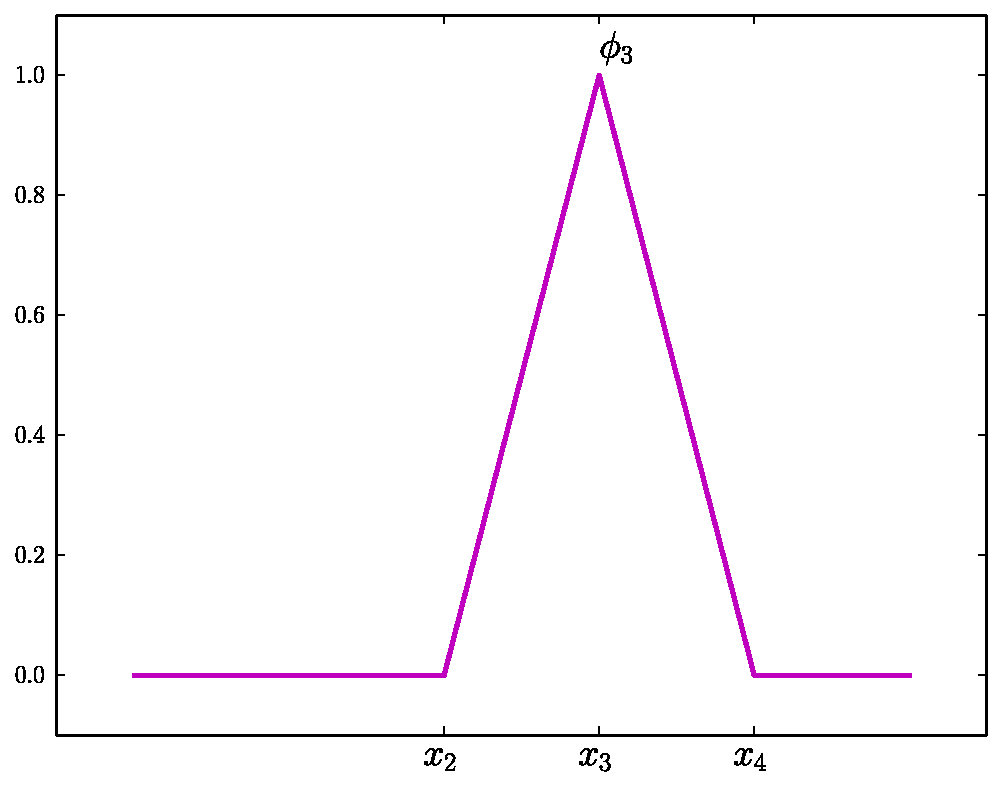
\includegraphics[width=\textwidth]{one_basis_function.pdf}
\caption{The basis function $\phi_3$.}
\label{FEM:one_basis_function}
\end{figure}


\begin{figure}[ht]
\centering
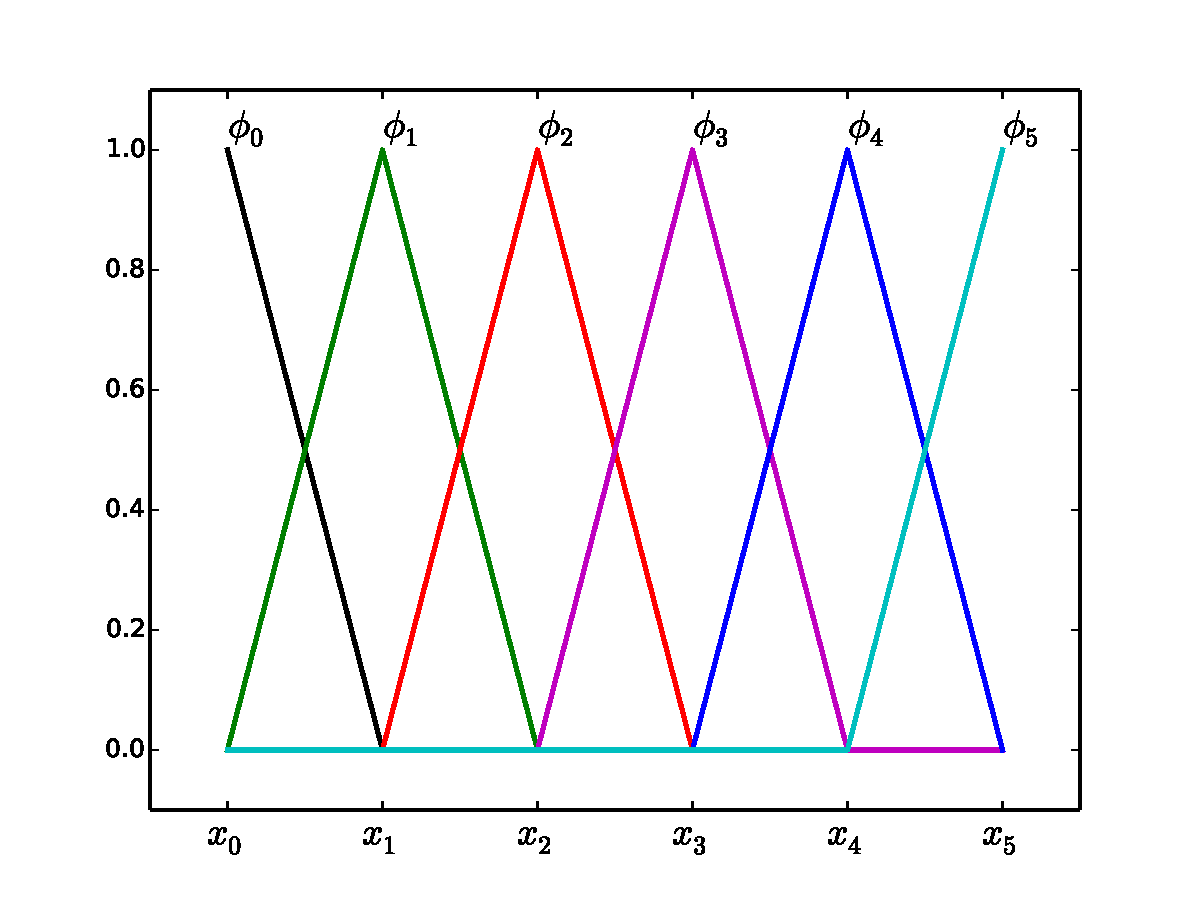
\includegraphics[width=\textwidth]{basis_functions.pdf}
\caption{Basis functions for $V_5$.}
\label{FEM:basis_functions}
\end{figure}





\begin{center}
  \begin{tabular}{ l |l l }
    % \hline
     & Finite Element & Finite Difference  \\ \hline
    Linear System& sparse& sparse  \\ 
   Derivative & approximated locally & approximated locally \\
Domain & irregular domains & Nice-ish\\
% Problem Formulation & integral & derivative & derivative & integral \\
Convergence & low order poly.& low order poly. \\
Strengths & adaptive mesh & easier to understand \\
&refinement & and implement \\
& complex geometries & \\
    \hline
  \end{tabular}
\end{center}


\begin{center}
  \begin{tabular}{ l |l l }
    % \hline
      & Pseudospectral & Finite Volume \\ \hline
    Linear System & dense & sparse \\ 
   Derivative & global & local\\
Domain  & Nice & Nice-ish\\
Convergence  & exponential & low order poly.\\
Strengths  & fast convergence & handling discontinuities \\
& accurate to high precisions & in the initial conditions \\
& & dealing with shock formation \\
& & and propagation \\
    \hline
  \end{tabular}
\end{center}

